\chapter{Fonctions usuelles}
\def\arraystretch{1}

\begin{definition}[Fonction polynomiale]
	Soient $n \in \N,\ a_0, \ldots, a_n \in \R$.
	\begin{center}
		$
		f :
		\begin{array}{|ccc}
			\R & \to & \R \\
             x & \mapsto & \sum_{i = 0}^{n} a_i x^i
		\end{array}
		$
	\end{center}
\end{definition}

\begin{definition}[Fonction partie entière]
	\[ \forall x \in \R,\ \exists ! E(x) \in \Z,\ E(x) \leq x < E(x + 1) \]
	\begin{center}
		$
		E :
		\begin{array}{|ccc}
			\R & \to & \Z \\
			x & \mapsto & E(x)
		\end{array}
		$
	\end{center}
\end{definition}

\begin{definition}[Fonction puissance]
	Soit $a \in \R$.
	\begin{center}
		$
		f :
		\begin{array}{|ccc}
			\R_+^* & \to & \R \\
			x & \mapsto & x^a
		\end{array}
		$
	\end{center}
\end{definition}

\begin{proposition}
	$\forall (a, b, x) \in \R^3$.
    \begin{multicols}{4}
        \begin{enumerate}
            \item $1^a = 1$.
            \item $x^a \cdot x^b = x^{a + b}$.
            \item $(xy)^a = x^a y^a$.
            \item $(x^a)^b = x^{ab}$.
        \end{enumerate}
    \end{multicols}
\end{proposition}

\section{Fonctions trigonométriques}
\begin{definition}[Fonctions trigonométriques]
	Pour tout $k \in \Z$ :	
	\begin{center}
		$
		\cos :
		\begin{array}{|ccc}
			 \R & \to & [-1, 1] \\
		      x & \mapsto & \cos(x)
		\end{array}
		\qquad
		\sin :
		\begin{array}{|ccc}
			 \R & \to & [-1, 1] \\
		      x & \mapsto & \sin(x)
		\end{array}
		\qquad
		\tan :
		\begin{array}{|ccc}
			 \R \backslash \left\{ \frac{k \pi}{2} \right\} & \to & \R \\ 
			  x & \mapsto & \frac{\sin(x)}{\cos(x)}
		\end{array}
		$
	\end{center}	
\end{definition}

\begin{figure}[h!]
	\centering
	%\includegraphics{images/cos.png}
	\begin{subfigure}{0.3\textwidth}
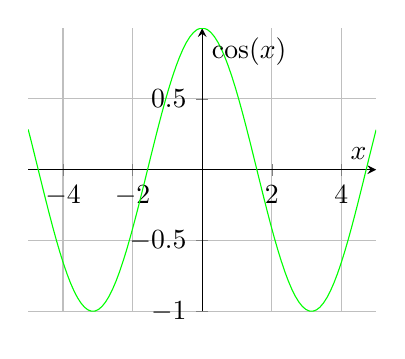
\begin{tikzpicture}
            \begin{axis}[domain=-5:5, axis lines=middle, grid=both, xlabel=$x$, ylabel=$\cos(x)$, width=6cm]
                \addplot[color=green, samples=100] {cos(deg(x))};
            \end{axis}
    \end{tikzpicture}
		
		\caption{Fonction $\cos{x}$}
	\end{subfigure}
	\begin{subfigure}{0.3\textwidth}
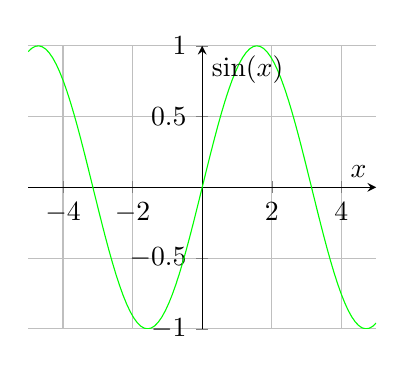
\begin{tikzpicture}
            \begin{axis}[domain=-5:5, axis lines=middle, grid=both, xlabel=$x$, ylabel=$\sin(x)$, width=6cm]
                \addplot[color=green, samples=100] {sin(deg(x))};
            \end{axis}
    \end{tikzpicture}
		\caption{Fonction $\sin{x}$}
	\end{subfigure}
	\begin{subfigure}{0.3\textwidth}
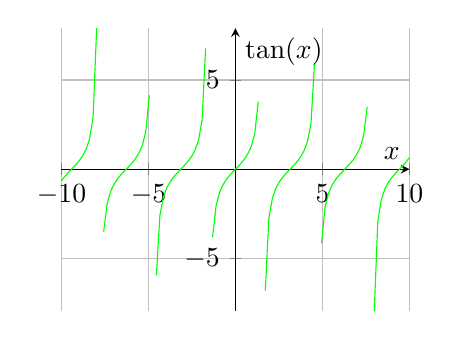
\begin{tikzpicture}
            \begin{axis}[domain=-10:10, restrict y to domain=-10:10, axis lines=middle, grid=both, xlabel=$x$, ylabel=$\tan(x)$, width=6cm]
                \addplot[color=green, samples=100] {tan(deg(x))};
            \end{axis}
    \end{tikzpicture}
		\caption{Fonction $\tan{x}$}
	\end{subfigure}
\end{figure}

\begin{figure}[h!]
	\centering
	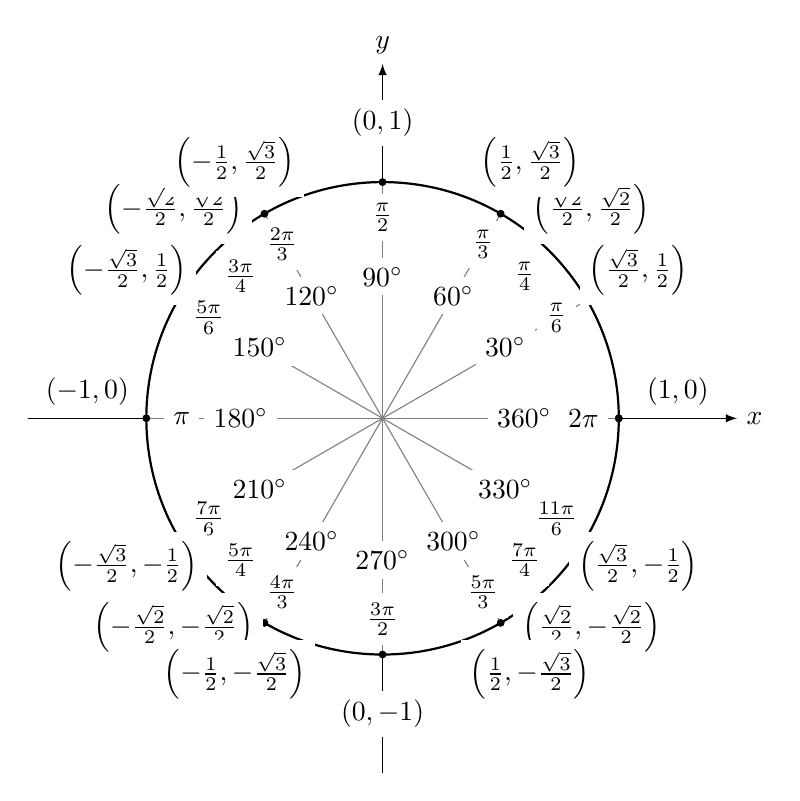
\begin{tikzpicture}[scale=3,cap=round,>=latex]
		% draw the coordinates
		\draw[->] (-1.5cm,0cm) -- (1.5cm,0cm) node[right,fill=white] {$x$};
		\draw[->] (0cm,-1.5cm) -- (0cm,1.5cm) node[above,fill=white] {$y$};
		
		% draw the unit circle
		\draw[thick] (0cm,0cm) circle(1cm);
		
		\foreach \x in {0,30,...,360} {
			% lines from center to point
			\draw[gray] (0cm,0cm) -- (\x:1cm);
			% dots at each point
			\filldraw[black] (\x:1cm) circle(0.4pt);
			% draw each angle in degrees
			\draw (\x:0.6cm) node[fill=white] {$\x^\circ$};
		}
		
		% draw each angle in radians
		\foreach \x/\xtext in {
			30/\frac{\pi}{6},
			45/\frac{\pi}{4},
			60/\frac{\pi}{3},
			90/\frac{\pi}{2},
			120/\frac{2\pi}{3},
			135/\frac{3\pi}{4},
			150/\frac{5\pi}{6},
			180/\pi,
			210/\frac{7\pi}{6},
			225/\frac{5\pi}{4},
			240/\frac{4\pi}{3},
			270/\frac{3\pi}{2},
			300/\frac{5\pi}{3},
			315/\frac{7\pi}{4},
			330/\frac{11\pi}{6},
			360/2\pi}
		\draw (\x:0.85cm) node[fill=white] {$\xtext$};
		
		\foreach \x/\xtext/\y in {
			% the coordinates for the first quadrant
			30/\frac{\sqrt{3}}{2}/\frac{1}{2},
			45/\frac{\sqrt{2}}{2}/\frac{\sqrt{2}}{2},
			60/\frac{1}{2}/\frac{\sqrt{3}}{2},
			% the coordinates for the second quadrant
			150/-\frac{\sqrt{3}}{2}/\frac{1}{2},
			135/-\frac{\sqrt{2}}{2}/\frac{\sqrt{2}}{2},
			120/-\frac{1}{2}/\frac{\sqrt{3}}{2},
			% the coordinates for the third quadrant
			210/-\frac{\sqrt{3}}{2}/-\frac{1}{2},
			225/-\frac{\sqrt{2}}{2}/-\frac{\sqrt{2}}{2},
			240/-\frac{1}{2}/-\frac{\sqrt{3}}{2},
			% the coordinates for the fourth quadrant
			330/\frac{\sqrt{3}}{2}/-\frac{1}{2},
			315/\frac{\sqrt{2}}{2}/-\frac{\sqrt{2}}{2},
			300/\frac{1}{2}/-\frac{\sqrt{3}}{2}}
		\draw (\x:1.25cm) node[fill=white] {$\left(\xtext,\y\right)$};
		
		% draw the horizontal and vertical coordinates
		% the placement is better this way
		\draw (-1.25cm,0cm) node[above=1pt] {$(-1,0)$}
		(1.25cm,0cm)  node[above=1pt] {$(1,0)$}
		(0cm,-1.25cm) node[fill=white] {$(0,-1)$}
		(0cm,1.25cm)  node[fill=white] {$(0,1)$};
	\end{tikzpicture}
	\caption{Cercle trigonométrique}
\end{figure}

\begin{proposition}
	$\forall x \in \R,\ k \in \Z$.
	\begin{enumerate}
		\item $\cos(-x) = \cos(x)$.
		\item $\sin(-x) = -\sin(x)$.
		\item $\tan(-x) = -\tan(x)$.
		\item $\cos(x + 2k\pi) = \cos(x)$.
		\item $\sin(x + 2k\pi) = \sin(x)$.
		\item $\tan(x + k\pi) = \tan(x)$.
		\item $\cos$ est bijective sur $[0, \pi]$.
		\item $\sin$ est bijective sur $[-\frac{\pi}{2}, \frac{\pi}{2}]$.
		\item $\tan$ est bijective sur $]-\frac{\pi}{2}, \frac{\pi}{2}[$.
	\end{enumerate}
\end{proposition}

\begin{definition}
	On définit $\arccos,\ \arcsin$ et $\arctan$ comme étant les bijections réciproques des fonctions $\cos,\ \sin$ et $\tan$.
\end{definition}

\begin{figure}[h!]
	\centering
	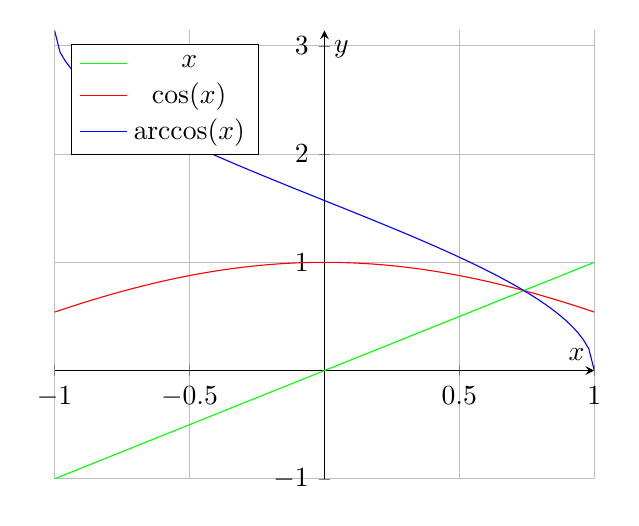
\begin{tikzpicture}
		\begin{axis}[domain=-1:1, axis lines=middle, grid=both, xlabel=$x$, ylabel=$y$, samples=100, legend pos=north west]
			\addplot[color=green]{x};
			\addlegendentry{$x$}
			\addplot[color=red]  {cos(deg(x))};
			\addlegendentry{$\cos(x)$}
			\addplot[color=blue]  {rad(acos(x))};
			\addlegendentry{$\arccos(x)$}
		\end{axis}
	\end{tikzpicture}
	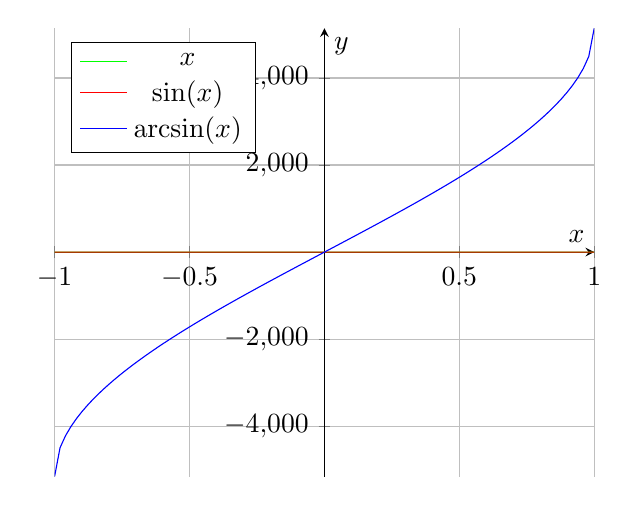
\begin{tikzpicture}
		\begin{axis}[domain=-1:1, axis lines=middle, grid=both, xlabel=$x$, ylabel=$y$, samples=100, legend pos=north west]
			\addplot[color=green]{x};
			\addlegendentry{$x$};
			\addplot[color=red]  {sin(deg(x))};
			\addlegendentry{$\sin(x)$};
			\addplot[color=blue]  {deg(asin(x))};
			\addlegendentry{$\arcsin(x)$};
		\end{axis}
	\end{tikzpicture}
	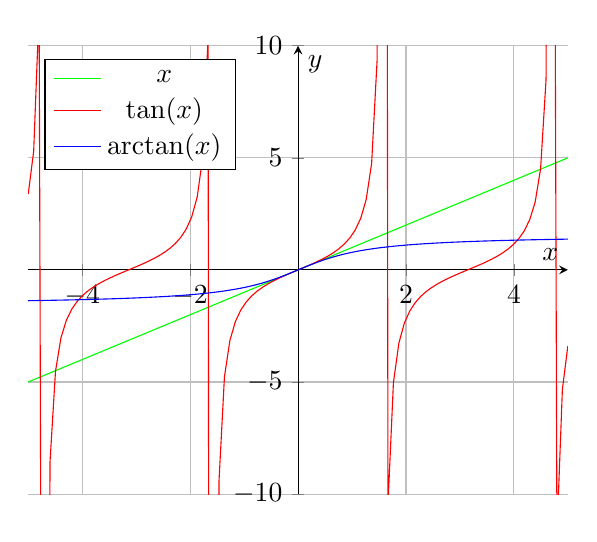
\begin{tikzpicture}
		\begin{axis}[xmin=-5, xmax=5, ymin=-10, ymax=10, axis lines=middle, grid=both, xlabel=$x$, ylabel=$y$, samples=100, legend pos=north west]
			\addplot[color=green]{x};
			\addlegendentry{$x$};
			\addplot[color=red]  {tan(deg(x))};
			\addlegendentry{$\tan(x)$};
			\addplot[color=blue]  {rad(atan(x))};
			\addlegendentry{$\arctan(x)$};
		\end{axis}
	\end{tikzpicture}
\end{figure}

\begin{proposition}
    \begin{enumerate}
    	\item $\forall x \in [-\frac{\pi}{2}, \frac{\pi}{2}],\ \arcsin(\sin(x)) = x$.
        \item $\forall x \in ]-\frac{\pi}{2}, \frac{\pi}{2}[,\ \arctan(\tan(x)) = x$.
        \item $\forall x \in [0, \pi],\ \arccos(\cos(x)) = x$.
        \item $\forall x \in [-1, 1]$ :
        \begin{multicols}{2}
            \begin{enumerate}
                \item $\sin(\arcsin(x)) = x$.
                \item $\cos(\arccos(x)) = x$.
            \end{enumerate}
        \end{multicols}
        \item $\forall x \in \R,\ \tan(\arctan(x)) = x$.
    \end{enumerate}
\end{proposition}

\begin{proposition}
	$\forall (a, b) \in \R^2$.
        \begin{enumerate}
            \item $\sin(a + b) = \sin(a) \cos(b) + \sin(b) \cos(a)$.
            \item $\cos(a + b) = \cos(a) \cos(b) - \sin(a) \sin(b)$.
        \end{enumerate}
\end{proposition}

\begin{proof}
    Nous pouvons procéder avec des produits scalaires, mais nous allons utiliser les nombres complexes ici.
    \\
    D'une part :
    \[e^{i (a + b)} = \cos(a + b) + i\sin(a + b)\]
    D'autre part :
    \begin{align*}
        e^{i (a + b)} &= e^{ia} \cdot e^{ib} \\
        &= [\cos(a) + i \sin(a)] \cdot [\cos(b) + i \sin(b)] \\
        &= \cos(a) \cos(b) + i\sin(b)\cos(a) + i\sin(a)\cos(b) - \sin(a)\sin(b) \\
        &= \cos(a)\cos(b) - \sin(a)\sin(b) + i [\sin(b)\cos(a) + \sin(a) \cos(b)].
    \end{align*}
    Par identification de la partie réelle et de la partie imaginaire :
    \[ \sin(a + b) = \sin(a) \cos(b) + \sin(b) \cos(a) \]
	\[ \cos(a + b) = \cos(a) \cos(b) - \sin(a) \sin(b) \]
\end{proof}

\begin{proposition}
    $\forall x \in \R,\ \cos^2(x) + \sin^2(x) = 1$.
\end{proposition}

\begin{proof}
    C'est une application du théorème de Pythagore sachant que le rayon du cercle trigonométrique est égal à 1.
\end{proof}

\begin{proposition}
	
    \begin{enumerate}
        \item $\lim_{x \to +\infty} \arctan(x) = \frac{\pi}{2}$.
        \item $\lim_{x \to -\infty} \arctan(x) = -\frac{\pi}{2}$.
    \end{enumerate}
\end{proposition}

\section{Exponentielle et logarithme}

\begin{definition}[Fonction exponentielle]
	\begin{center}
		$
		\exp : 
		\begin{array}{|ccc}
			\R & \to & \R_+^* \\
			x & \mapsto & \exp(x) \equiv e^x
		\end{array}
		$
	\end{center}
\end{definition}

\begin{proposition}
	La fonction exponentielle est \textbf{bijective} et \textbf{strictement croissante} et $\exp(0) = 1$.
    \begin{multicols}{2}
        \begin{enumerate}
            \item $\lim_{x \to -\infty} e^x = 0$.
            \item $\lim_{x \to +\infty} e^x = +\infty$.
        \end{enumerate}
    \end{multicols}
    \noindent $\forall (x, y) \in \R^2$.
    \begin{multicols}{2}
        \begin{enumerate}
            \item $\exp(x + y) = \exp(x) \cdot \exp(y)$.
            \item $\exp(-x) = \frac{1}{\exp(x)}$.
            \item $\exp(x - y) = \frac{\exp(x)}{\exp(y)}$.
        \end{enumerate}
    \end{multicols}
\end{proposition}

\begin{definition}[Logarithme néperien]
	\begin{center}
		$
		\ln : 
		\begin{array}{|ccc}
			\R_+^* & \to & \R \\
			x & \mapsto & \ln(x)
		\end{array}
		$
	\end{center}
\end{definition}

\begin{figure}[!h]
	\centering
	\begin{subfigure}{0.45\textwidth}
		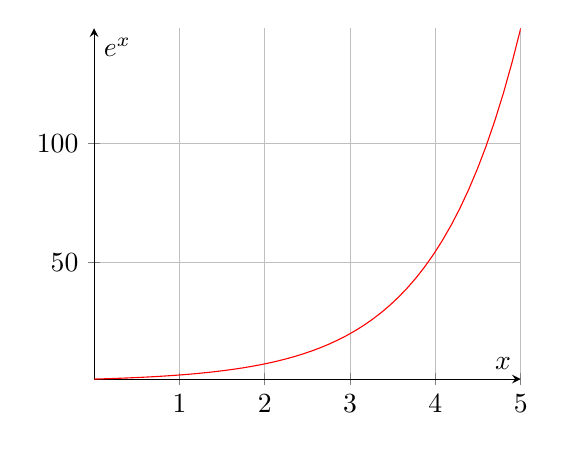
\begin{tikzpicture}
			\begin{axis}[domain=0:5, axis lines=middle, grid=both, xlabel=$x$, ylabel=$e^x$, width=7cm]
				\addplot[color=red, samples=50]{e^x};
			\end{axis}
		\end{tikzpicture}  
		\caption{Fonction exponentielle}
	\end{subfigure}
	\begin{subfigure}{0.45\textwidth}
		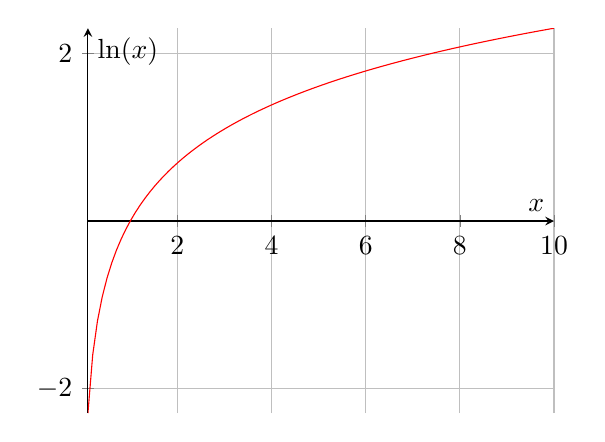
\begin{tikzpicture}
			\begin{axis}[domain=0:10, axis lines=middle, grid=both, xlabel=$x$, ylabel=$\ln(x)$, width=7.5cm]
				\addplot[color=red, samples=100]{ln(x)};
			\end{axis}
		\end{tikzpicture}
		\caption{Fonction logarithme népérien}
	\end{subfigure}
\end{figure}

\begin{proposition}
	$\forall (x, y) \in \R_+^* \times \R$.
    \begin{multicols}{2}
        \begin{enumerate}
            \item $\exp(\ln(x)) = x$.
            \item $\ln(\exp(y)) = y$.
        \end{enumerate}
    \end{multicols}
\end{proposition}

\begin{proposition}
	La fonction logarithme néperien est \textbf{bijective} et \textbf{strictement croissante} et $\ln(1) = 0$.
    \begin{multicols}{2}
        \begin{enumerate}
            \item $\lim_{x \to 0} \ln(x) = -\infty$.
            \item $\lim_{x \to +\infty} \ln(x) = +\infty$.
        \end{enumerate}
    \end{multicols}
    \noindent $\forall (x, y) \in \R^2$.
    \begin{multicols}{2}
        \begin{enumerate}
            \item $\ln(xy) = \ln(x) + \ln(y)$.
            \item $\ln(\frac{1}{x}) = -\ln(x)$.
            \item $\ln(\frac{x}{y}) = \ln(x) - \ln(y)$.
            \item $\ln(x^n) = n\ln(x)$.
        \end{enumerate}
    \end{multicols}
\end{proposition}

\section{Fonctions hyperboliques}

\begin{definition}[Fonctions hyperboliques]
	
	\begin{center}
		$
		\cosh :
		\begin{array}{|ccc}
			\R & \to & \R \\
		         x & \mapsto & \frac{e^x + e^{-x}}{2}
		\end{array}
		\qquad 
		\sinh :
		\begin{array}{|ccc}
			\R & \to & \R \\ 
			     x & \mapsto & \frac{e^x - e^{-x}}{2}
		\end{array}
		\qquad
		\tanh : 
		\begin{array}{|ccc}
			\R & \to & \R \\ 
				 x & \mapsto & \frac{\sinh(x)}{\cosh(x)} = \frac{e^x - e^{-x}}{e^x + e^{-x}}
		\end{array}
		$
	\end{center}
\end{definition}

\begin{figure}[!h]
	\centering
	\begin{subfigure}{0.3\textwidth}
		%\includegraphics[width=\textwidth, height=3.5cm]{images/ch.png}
		
		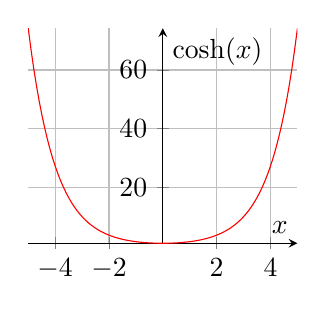
\begin{tikzpicture}
			\begin{axis}[domain=-5:5, axis lines=middle, grid=both, xlabel=$x$, ylabel=$\cosh(x)$, width=5cm]
				\addplot[color=red, samples=100]  {cosh(x)};
			\end{axis}
		\end{tikzpicture}
		\caption{Fonction cosh}
	\end{subfigure}
	\begin{subfigure}{0.3\textwidth}
		%\includegraphics[width=\textwidth, height=3.5cm]{images/sh.png}
		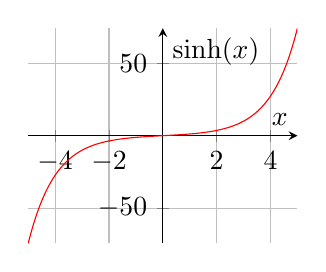
\begin{tikzpicture}
			\begin{axis}[domain=-5:5, axis lines=middle, grid=both, xlabel=$x$, ylabel=$\sinh(x)$, width=5cm]
				\addplot[color=red, samples=100]  {sinh(x)};
			\end{axis}
		\end{tikzpicture}
		\caption{Fonction sinh}
	\end{subfigure}
	\begin{subfigure}{0.3\textwidth}
		%\includegraphics[width=\textwidth, height=3.5cm]{images/tanh.png}
		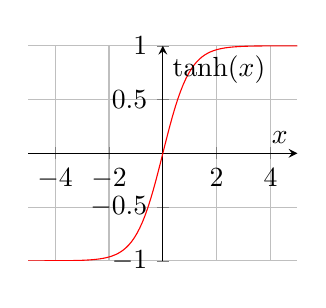
\begin{tikzpicture}
			\begin{axis}[domain=-5:5, axis lines=middle, grid=both, xlabel=$x$, ylabel=$\tanh(x)$, width=5cm]
				\addplot[color=red, samples=100]  {tanh(x)};
			\end{axis}
		\end{tikzpicture}
		\caption{Fonction tanh}
	\end{subfigure}
\end{figure}

\begin{proposition}
	$\forall (x,k) \in \R \times \Z$.
	\begin{enumerate}
		\item $\cosh(-x) = \cosh(x)$.
		\item $\sinh(-x) = \sinh(x)$.
		\item $\tanh(-x) = \tanh(x)$.
	\end{enumerate}
\end{proposition}

\begin{proposition}
	$\forall (x, y) \in \R^2$.
    \begin{enumerate}
        \item $\cosh(x + y) = \cosh(x) \cosh(y) + \sinh(x) \sinh(y)$.
        \item $\sinh(x + y) = \cosh(x) \sinh(y) + \sinh(x) \cosh(y)$.
    \end{enumerate}
\end{proposition}

\begin{proof}
    Calcul direct avec les définitions de $\cosh$ et de $\sinh$.
\end{proof}
